\documentclass[11pt]{article}

\usepackage[margin=1in]{geometry}
\usepackage{amsmath}
\usepackage{booktabs}
\usepackage{graphicx}
\usepackage{float}
\usepackage{hyperref}

\graphicspath{{figures/}}

\title{Baseline Heavy-Ball Extremum Seeking Control on Multiple Cost Functions}
\author{Matt}
\date{\today}

\begin{document}
\maketitle

\section{Introduction}

This report evaluates the baseline Heavy-Ball extremum seeking controller
without Gaussian fill or PDE escape extensions. The goal is to test how the
controller behaves on quadratic, quartic, plateau-like, and multi-basin cost
functions, with special attention to robot speed limits and local escape.

All reported runs use:
\[
\texttt{use\_pde\_extensions}=\texttt{False}, \qquad
\texttt{escape\_policy}=\texttt{none}.
\]

\section{Method}

The TurtleBot simulation used a rotating sensor and the baseline Heavy-Ball
controller. The Heavy-Ball tuning was held fixed:
\[
k_{vx}=0.2, \quad k_{wz}=2.0, \quad k=1.0, \quad
\beta=0.1, \quad \texttt{input\_gain}=-1.0.
\]

The physical-speed controller used the TurtleBot wheel limit:
\[
v_{x,\max}=0.2419\ \mathrm{m/s}, \qquad
\omega_{z,\max}=0.75\ \mathrm{rad/s}.
\]
The slow and fast cases were used only to study the effect of speed limits.
The fast case is simulation-only and should not be interpreted as a physically
valid TurtleBot setting.

\subsection{Cost Functions}

The quadratic bowl was
\[
J_q(x,y)=0.05\left((x-10)^2+(y-10)^2\right).
\]

The quartic bowl was
\[
J_r(x,y)=0.0005\left((x-10)^4+(y-10)^4\right).
\]

The quartic double-well map used
\[
u=\frac{x+y}{2}
\]
and
\[
J_w(x,y)=0.01(u-2)^2(u-10)^2+0.0125(x-y)^2-0.005u.
\]

The Gaussian two-basin maps were the original \texttt{2D\_local\_min.json}
and the widened-global-basin \texttt{2D\_local\_min\_globalW40.json}.

\section{Test Matrix}

\begin{table}[H]
\centering
\begin{tabular}{lllll}
\toprule
ID & Cost map & Start & Speed & Purpose \\
\midrule
Q1 & Quadratic bowl & $(0,0)$ & real & convex convergence \\
Q2 & Quadratic bowl & $(6,6)$ & real & medium start \\
Q3 & Quadratic bowl & $(8,8)$ & real & near-minimum behavior \\
R1 & Quartic bowl & $(0,0)$ & real & far quartic start \\
R2 & Quartic bowl & $(6,6)$ & real & medium quartic start \\
R3 & Quartic bowl & $(8,8)$ & real & plateau-like behavior \\
W1 & Quartic double-well & $(1,1)$ & slow & low-speed escape \\
W2 & Quartic double-well & $(1,1)$ & real & physical-speed escape \\
W3 & Quartic double-well & $(1,1)$ & fast & simulation-only speed test \\
G1 & globalW40 & $(1,1)$ & slow & known easier escape map \\
G2 & globalW40 & $(1,1)$ & real & physical-speed benchmark \\
G3 & globalW40 & $(1,1)$ & fast & simulation-only speed test \\
H1 & original two-basin & $(0,0)$ & slow & hard-map low speed \\
H2 & original two-basin & $(0,0)$ & real & hard-map physical speed \\
H3 & original two-basin & $(0,0)$ & fast & hard-map simulation-only speed \\
\bottomrule
\end{tabular}
\caption{Focused baseline Heavy-Ball test matrix.}
\end{table}

\section{Quadratic vs. Quartic Results}

Table~\ref{tab:single-well-results} summarizes the single-well tests. The
quadratic and quartic bowl cases both moved toward the minimizer at $(10,10)$.
The final distance was not exactly zero because the controller continued to
dither and circle near the minimum, but all six tests entered the target
neighborhood.

\begin{table}[H]
\centering
\resizebox{\textwidth}{!}{%
\begin{tabular}{llllllll}
\toprule
ID & Start & Duration [s] & Final $(x,y)$ & Tail dist. [m] & Final cost & $v_x$ sat. & Observation \\
\midrule
Q1 & $(0,0)$ & 379.6 & $(10.37,10.49)$ & 0.63 & 0.0121 & 37\% & reached target neighborhood \\
Q2 & $(6,6)$ & 277.8 & $(9.92,10.65)$ & 0.67 & 0.0200 & 31\% & reached target neighborhood \\
Q3 & $(8,8)$ & 260.2 & $(9.48,10.35)$ & 0.64 & 0.0255 & 10\% & reached target neighborhood \\
R1 & $(0,0)$ & 516.3 & $(10.00,10.54)$ & 0.56 & $1.04{\times}10^{-5}$ & 24\% & reached target neighborhood \\
R2 & $(6,6)$ & 463.0 & $(10.54,9.79)$ & 0.59 & $1.62{\times}10^{-5}$ & 2\% & reached target neighborhood \\
R3 & $(8,8)$ & 212.0 & $(9.67,9.22)$ & 0.88 & $4.05{\times}10^{-4}$ & 0\% & slowest near-minimum case \\
\bottomrule
\end{tabular}}
\caption{Single-well quadratic and quartic results. Tail distance is the mean
distance to $(10,10)$ over the final 30 seconds of the run.}
\label{tab:single-well-results}
\end{table}

The quadratic bowl tests saturated the forward velocity more often when the
robot started farther from the target. For example, Q1 saturated $v_x$ for
37\% of the logged control samples, while Q3 saturated for only 10\%. In the
quartic tests, the far-start case R1 still saturated for 24\%, but the
near-start case R3 had no velocity saturation and much smaller control
commands. This is consistent with the quartic cost becoming very flat near the
minimum.

\section{Plateau Discussion}

The quartic bowl has a flatter gradient near the minimum than the quadratic
bowl. This appeared most clearly in R3. The robot started at $(8,8)$, so it was
already near the minimizer, but the local quartic gradient was small. The
controller did not hit the speed limits, with maximum values
$|v_x|=0.0326$ m/s and $|\omega_z|=0.1115$ rad/s, far below the physical caps.
The final 30-second mean distance to $(10,10)$ was 0.88 m, larger than the
corresponding quadratic near-start case Q3 at 0.64 m.

This supports the expected plateau behavior: a flatter cost provides weaker
gradient information to the ESC filter, so the controller can remain active but
make slow progress near the optimum.

\begin{figure}[H]
\centering
\begin{minipage}{0.48\textwidth}
\centering
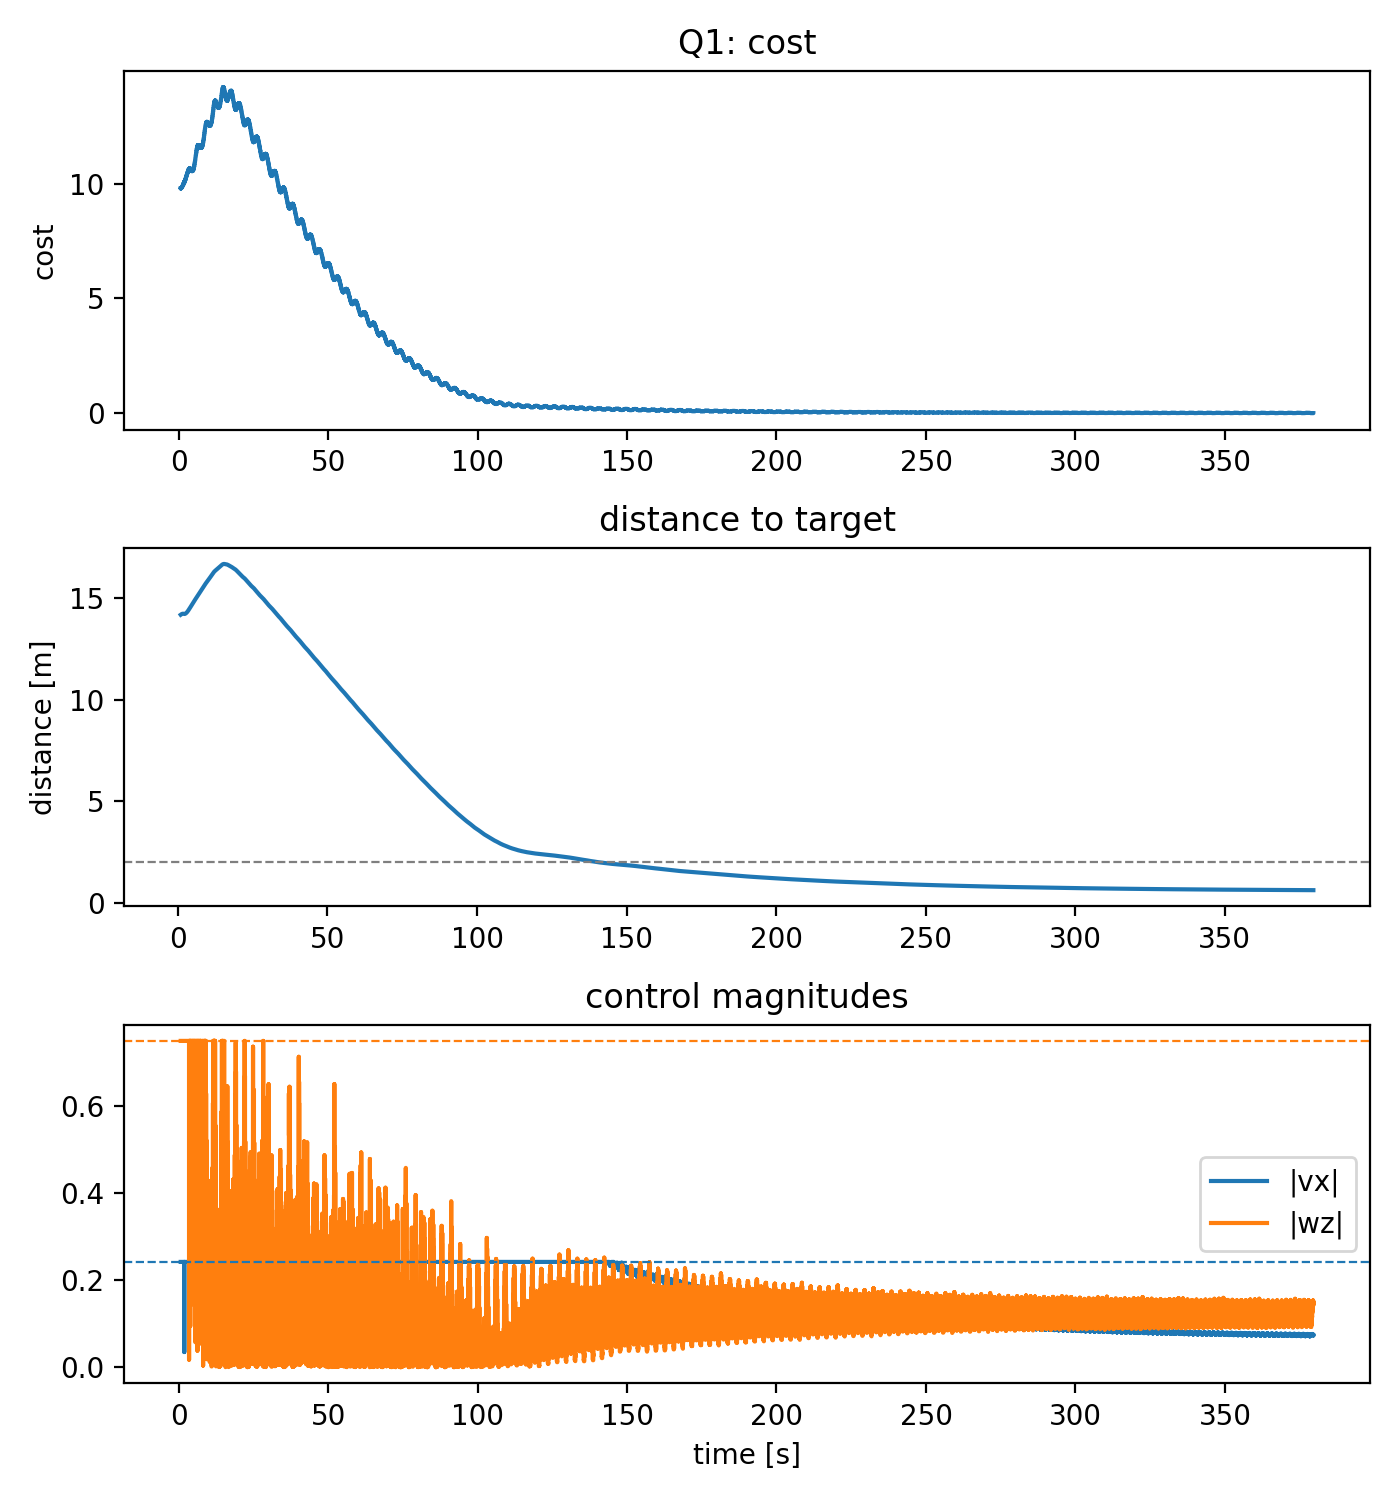
\includegraphics[width=\linewidth]{Q1_timeseries.png}
\caption{Quadratic far-start time histories.}
\label{fig:q1-timeseries}
\end{minipage}
\hfill
\begin{minipage}{0.48\textwidth}
\centering
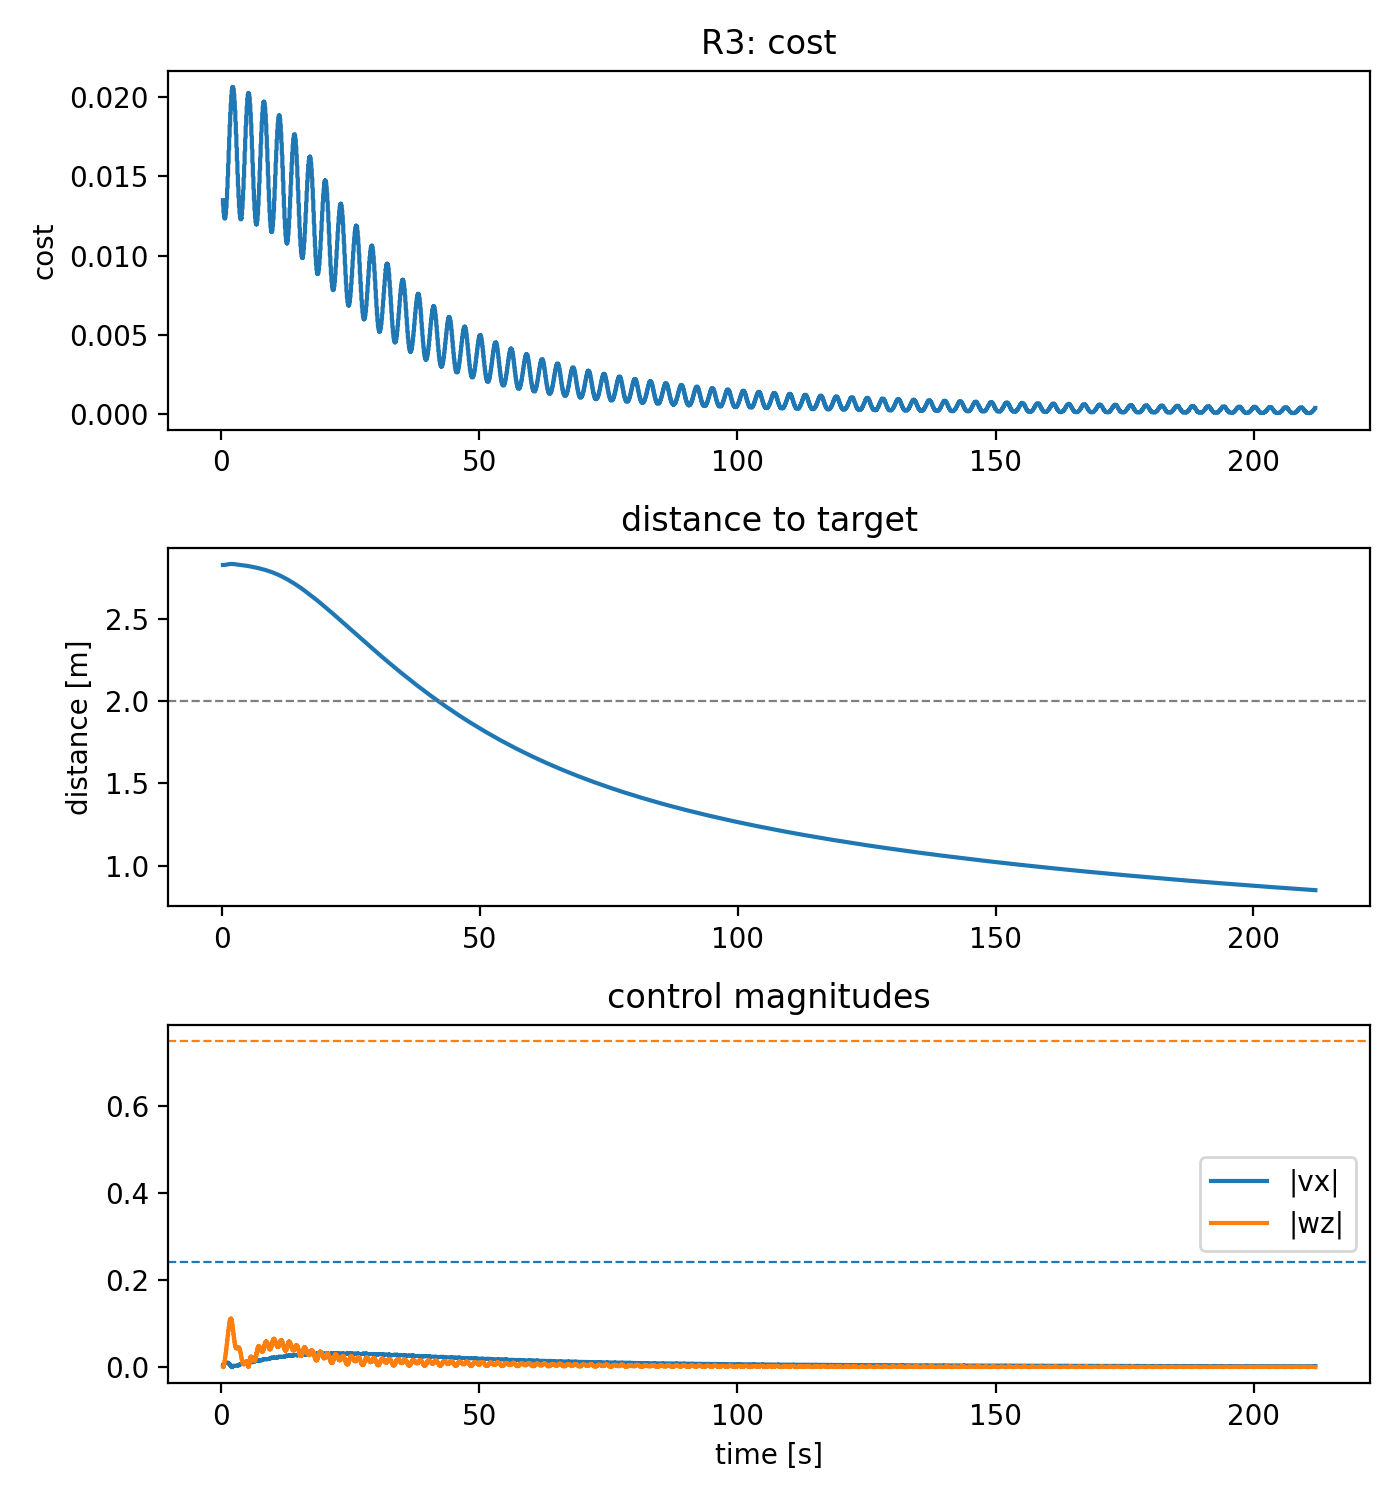
\includegraphics[width=\linewidth]{R3_timeseries.png}
\caption{Quartic near-start time histories.}
\label{fig:r3-timeseries}
\end{minipage}
\end{figure}

\section{Local Escape and Speed Limits}

Table~\ref{tab:escape-results} summarizes the two-basin and double-well tests.
The global target is the basin near $(10,10)$ and the local basin is near
$(2,2)$.

\begin{table}[H]
\centering
\resizebox{\textwidth}{!}{%
\begin{tabular}{llllllll}
\toprule
ID & Map & Speed & Duration [s] & Final $(x,y)$ & Tail dist. [m] & $v_x$ sat. & Local/global outcome \\
\midrule
G1 & globalW40 & slow & 271.6 & $(2.73,3.07)$ & 10.41 & 99\% & remained near local basin \\
G2 & globalW40 & real & 281.5 & $(9.11,8.87)$ & 1.40 & 99\% & escaped and reached global basin \\
G3 & globalW40 & fast & 153.9 & $(12.16,10.41)$ & 2.26 & 100\% & escaped but circled wide \\
H1 & original & slow & 200.2 & $(1.75,1.72)$ & 11.25 & 100\% & trapped near local basin \\
H2 & original & real & 638.4 & $(0.57,1.98)$ & 11.04 & 100\% & did not reach global basin \\
H3 & original & fast & 313.5 & $(0.43,3.65)$ & 11.22 & 100\% & did not reach global basin \\
W1 & quartic double-well & slow & 242.9 & $(2.15,1.96)$ & 11.32 & 58\% & trapped near local basin \\
W2 & quartic double-well & real & 173.1 & $(2.08,2.03)$ & 11.30 & 20\% & trapped near local basin \\
W3 & quartic double-well & fast & 151.7 & $(2.17,2.08)$ & 11.28 & 14\% & trapped near local basin \\
\bottomrule
\end{tabular}}
\caption{Local escape and speed-limit results. The tail distance is measured
relative to the global basin at $(10,10)$.}
\label{tab:escape-results}
\end{table}

The clearest speed-limit effect occurred on the widened-global-basin map
\texttt{globalW40}. With the slow speed cap, G1 stayed near the local basin and
never reached the global basin. With the physical TurtleBot speed cap, G2
escaped the local basin quickly and reached the global basin. With the
simulation-only fast speed cap, G3 escaped the local basin but overshot and
settled into a wider orbit around the global region. Therefore, increasing the
speed limit can improve local escape, but excessive speed does not necessarily
improve final convergence quality.

The original Gaussian two-basin map was harder. H1--H3 all failed to reach the
global basin, even though the controller saturated the forward velocity for
nearly the entire run. This suggests that speed saturation alone is not enough:
the local cost geometry and the Heavy-Ball dynamics still determine whether the
robot can build useful escape momentum.

The quartic double-well tests W1--W3 were also trapped near $(2,2)$. In this
case, increasing the speed limit did not help. The real and fast cases actually
showed less forward-velocity saturation than W1, which indicates that the
polynomial local basin and plateau-like structure provided insufficient
directional information for escape.

\begin{figure}[H]
\centering
\begin{minipage}{0.48\textwidth}
\centering
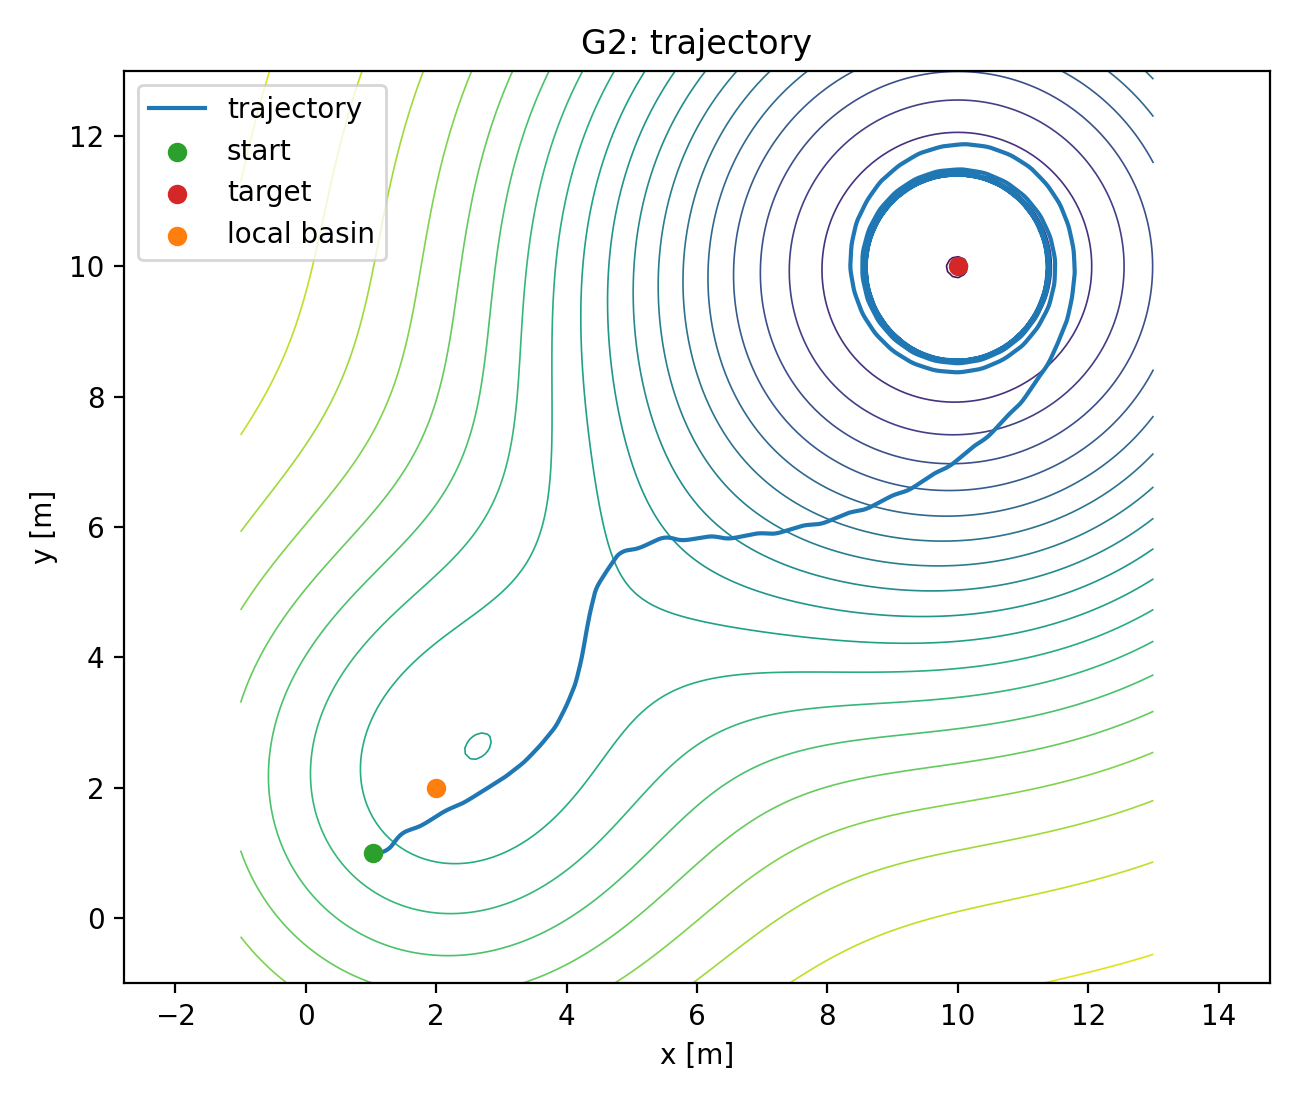
\includegraphics[width=\linewidth]{G2_trajectory.png}
\caption{G2 trajectory: physical-speed escape on \texttt{globalW40}.}
\label{fig:g2-trajectory}
\end{minipage}
\hfill
\begin{minipage}{0.48\textwidth}
\centering
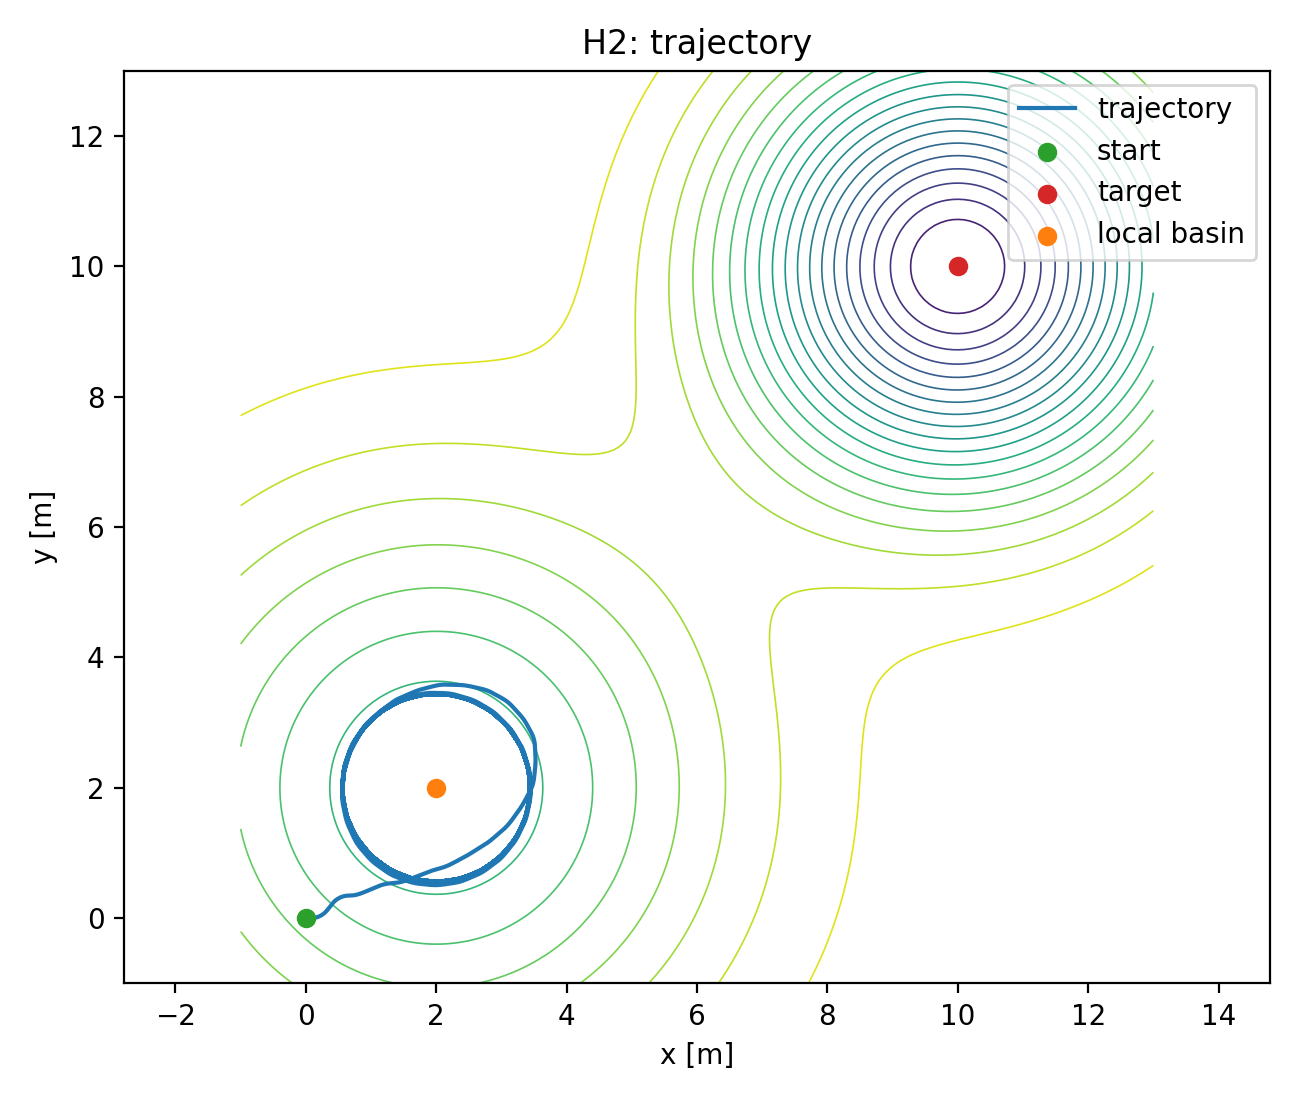
\includegraphics[width=\linewidth]{H2_trajectory.png}
\caption{H2 trajectory: original map did not reach the global basin.}
\label{fig:h2-trajectory}
\end{minipage}
\end{figure}

\begin{figure}[H]
\centering
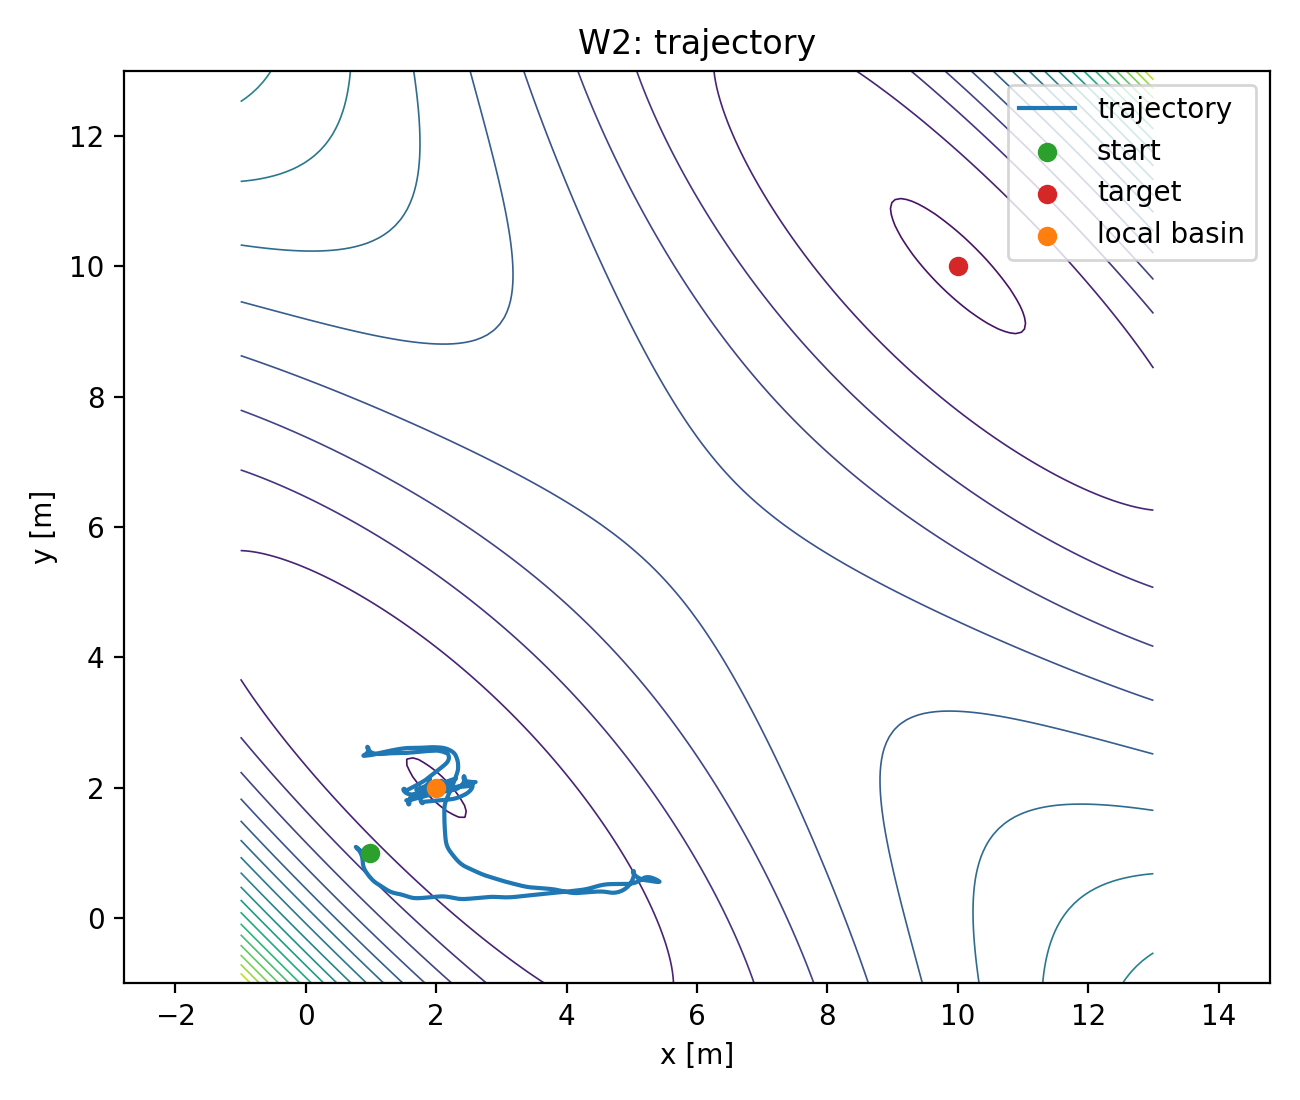
\includegraphics[width=0.65\textwidth]{W2_trajectory.png}
\caption{W2 trajectory: quartic double-well with physical speed limits trapped
near the local basin.}
\label{fig:w2-trajectory}
\end{figure}

\section{Findings}

\begin{itemize}
  \item Baseline Heavy-Ball ESC handled the single-well quadratic and quartic
        maps, but it converged to a bounded orbit rather than an exact point.
  \item The quartic bowl showed plateau effects near the minimum: smaller
        controls, little speed saturation, and slower progress in the near-start
        case.
  \item Speed limits strongly affected escape on \texttt{globalW40}. Slow speed
        failed, physical speed escaped, and fast simulation-only speed escaped
        but circled farther from the global minimum.
  \item The original two-basin map remained difficult. Even real and fast
        speed-limit cases did not reach the global basin.
  \item The quartic double-well trapped the robot near $(2,2)$ for all tested
        speed limits, showing that some local minima cannot be handled by
        baseline Heavy-Ball momentum alone.
  \item Gaussian fills remain useful when baseline Heavy-Ball cannot escape a
        local basin by momentum alone.
\end{itemize}

\section{Conclusion}

The baseline Heavy-Ball algorithm was effective on smooth single-well costs and
could escape the widened-global-basin map when the physical TurtleBot speed
limit was available. However, it did not reliably solve harder local-minimum
maps. The original Gaussian two-basin map and the quartic double-well both
demonstrated failure cases where the robot remained trapped or failed to reach
the global basin without Gaussian fill.

The speed-limit tests show that local escape depends on both available velocity
and cost-map geometry. More speed can help in some maps, but speed alone is not
a complete solution. Plateau-like costs and strong local basins reduce the
effective gradient information available to the ESC controller, which motivates
the Gaussian-fill extension for future global-seeking experiments.

\appendix
\section{Run and Analysis Commands}

Preview all baseline scenarios:
\begin{verbatim}
bash ~/dsim-lab/ros2_ws/src/turtlebot3_rotating_sensor/bash_scripts/\
accelerated_methods/hb_baseline_matrix_acoustic.bash --dry-run
\end{verbatim}

Run one scenario:
\begin{verbatim}
bash ~/dsim-lab/ros2_ws/src/turtlebot3_rotating_sensor/bash_scripts/\
accelerated_methods/hb_scenario_acoustic.bash \
~/dsim-lab/ros2_ws/src/ros_esc/paper_recreations/heavy_ball_PDE_ESC/\
scenarios/baseline_tests/Q1_quadratic_start0_real.json
\end{verbatim}

After filling in \texttt{report/baseline\_hb\_run\_manifest.csv}, analyze
completed runs:
\begin{verbatim}
python3 ~/dsim-lab/ros2_ws/src/ros_esc/paper_recreations/\
heavy_ball_PDE_ESC/analysis/analyze_baseline_hb_logs.py --plots
\end{verbatim}

The complete metrics table is saved at:
\begin{verbatim}
~/dsim-lab/ros2_ws/src/ros_esc/paper_recreations/heavy_ball_PDE_ESC/
report/baseline_hb_metrics.csv
\end{verbatim}

All generated figures are saved under:
\begin{verbatim}
~/dsim-lab/ros2_ws/src/ros_esc/paper_recreations/heavy_ball_PDE_ESC/
report/figures/
\end{verbatim}

\end{document}
